\documentclass[11pt,aspectratio=169]{beamer}

\usepackage[spanish,es-nodecimaldot]{babel}
\usepackage[utf8]{inputenc}
\usepackage[T1]{fontenc}
\usepackage{amsmath,amssymb}
\usepackage{graphicx}
\usepackage{booktabs}

\graphicspath{{../figuras/}}

% Estética sobria: tema por defecto, sin símbolos de navegación, número de diapo abajo
\usetheme{default}
\setbeamertemplate{navigation symbols}{}
\setbeamercolor{structure}{fg=black}
\setbeamertemplate{itemize items}{--}
\setbeamertemplate{footline}{\hfill\insertframenumber\,/\,\inserttotalframenumber\hspace{1em}\vspace{0.6em}}

\title{Posición de un motor de CC}
\subtitle{Control por realimentación de estados}
\author{Tomás Gómez Pizarro \and Mikael Rodríguez}
\institute{Sistemas de Control · FAMAF\\Proyecto parcial 2 · Variante 4 · Grupo 2}
\date{2026}

\begin{document}

% 1 -----------------------------------------------------------------------
\begin{frame}[plain]
  \begin{columns}[c]
    \begin{column}{0.5\textwidth}
      \centering
      {\Large \inserttitle\par}
      \vspace{0.4em}
      {\insertsubtitle\par}
      \vspace{1.5em}
      Tomás Gómez Pizarro\\Mikael Rodríguez\par
      \vspace{1.5em}
      {\small Sistemas de Control · FAMAF\\Proyecto parcial 2 · Variante 4 · Grupo 2\\2026\par}
    \end{column}
    \begin{column}{0.48\textwidth}
      \centering
      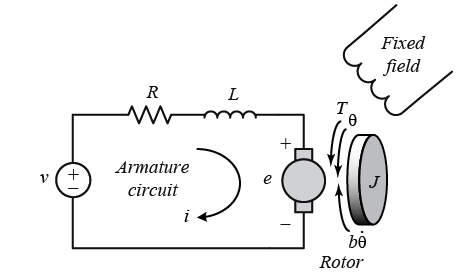
\includegraphics[width=\linewidth]{motor_cc_ctms.png}\\[0.2em]
      {\tiny Esquema: CTMS, \emph{DC Motor Position: System Modeling}}
    \end{column}
  \end{columns}
\end{frame}

% 2 -----------------------------------------------------------------------
\begin{frame}{El problema}
  Un motor de CC mueve una carga inercial. Hay que llevar el eje a una posición
  lo más rápido posible sin superar la tensión de la fuente.

  \vspace{0.8em}
  \begin{columns}[T]
    \begin{column}{0.5\textwidth}
      \textbf{Ecuaciones (dato)}
      \begin{align*}
        J\ddot\theta + b\dot\theta &= K\,i\\
        L\,\frac{di}{dt} + R\,i &= V - K\dot\theta
      \end{align*}
      \small
      \begin{tabular}{@{}ll@{}}
        $J = 5\times10^{-6}$ kg\,m$^2$ & $b = 4\times10^{-6}$ N\,m\,s\\
        $K = 0{,}03$ N\,m/A & $R = 3\ \Omega$\\
        $L = 0{,}4$ mH &
      \end{tabular}
    \end{column}
    \begin{column}{0.45\textwidth}
      \textbf{Condiciones}
      \begin{itemize}
        \item Se miden $\theta$, $\dot\theta$ e $i$.
        \item $|V| \le 12$ V.
      \end{itemize}
      \vspace{0.5em}
      \textbf{Especificaciones} (escalón de 1 rad)
      \begin{itemize}
        \item $T_s \le 50$ ms
        \item $PO \le 5$\,\%
        \item $e_{ss} = 0$
      \end{itemize}
    \end{column}
  \end{columns}
\end{frame}

% 3 -----------------------------------------------------------------------
\begin{frame}{Modelo en espacio de estados}
  \begin{columns}[T]
    \begin{column}{0.42\textwidth}
      \textbf{Estados}, entrada y salida
      \[
        x=\begin{bmatrix}\theta\\ \dot\theta\\ i\end{bmatrix}
        \begin{array}{l}
          \text{posición del eje [rad]}\\
          \text{velocidad del eje [rad/s]}\\
          \text{corriente de armadura [A]}
        \end{array}
      \]
      \[
        u = V,\qquad y = \theta
      \]
      \small
      $\dot\theta$ e $i$ salen de las dos ecuaciones diferenciales (mecánica y eléctrica);
      $\theta$ se agrega porque la salida es la posición.
    \end{column}
    \begin{column}{0.55\textwidth}
      \[
        A=\begin{bmatrix}0&1&0\\0&-\frac{b}{J}&\frac{K}{J}\\[2pt]0&-\frac{K}{L}&-\frac{R}{L}\end{bmatrix}
         =\begin{bmatrix}0&1&0\\0&-0{,}8&6000\\0&-75&-7500\end{bmatrix}
      \]
      \[
        B=\begin{bmatrix}0\\0\\\frac{1}{L}\end{bmatrix}=\begin{bmatrix}0\\0\\2500\end{bmatrix}
      \]
      \[
        C=\begin{bmatrix}1&0&0\end{bmatrix},\qquad D=0
      \]
      \small
      Misma estructura que el modelo del CTMS (\emph{DC Motor Position: System Modeling}),
      con otros parámetros.
    \end{column}
  \end{columns}
\end{frame}

% 4 -----------------------------------------------------------------------
\begin{frame}{Análisis: polos, estabilidad y controlabilidad}
  \textbf{Polos de lazo abierto} (autovalores de $A$)
  \[
    s_1 = 0,\qquad s_2 = -61{,}3,\qquad s_3 = -7439{,}5
  \]
  \begin{itemize}
    \item Polo simple en el origen: la posición integra la velocidad.
    \item Los otros dos en el semiplano izquierdo: mecánico ($-61{,}3$) y eléctrico ($-7439{,}5$).
    \item \textbf{Marginalmente estable}: ante una tensión constante $\theta$ crece sin límite.
  \end{itemize}

  \vspace{0.6em}
  \textbf{Controlabilidad}
  \[
    P_c=\begin{bmatrix}B & AB & A^2B\end{bmatrix},\qquad
    \det(P_c) = -5{,}625\times10^{17}\neq 0
  \]
  \begin{itemize}
    \item El sistema es \textbf{controlable}: con $V=-Kx+Nr$ se pueden ubicar los tres polos donde se quiera.
  \end{itemize}
\end{frame}

% 5 -----------------------------------------------------------------------
\begin{frame}{Diseño: elección de los polos}
  Se elige \textbf{ubicación de polos}: las especificaciones se traducen directo a $\zeta$ y $\omega_n$.

  \vspace{0.6em}
  \begin{columns}[T]
    \begin{column}{0.5\textwidth}
      \textbf{Par dominante}
      \begin{itemize}
        \item $PO \le 5$\,\% $\Rightarrow \zeta \ge 0{,}69$. Se toma $\zeta = 0{,}8$.
        \item $T_s \approx \dfrac{4}{\zeta\omega_n} \le 50$ ms $\Rightarrow \zeta\omega_n \ge 80$. Se toma $\omega_n = 110$ rad/s.
      \end{itemize}
      \[
        s_{1,2} = -\zeta\omega_n \pm j\,\omega_n\sqrt{1-\zeta^2} = -88 \pm j\,66
      \]
    \end{column}
    \begin{column}{0.45\textwidth}
      \textbf{Tercer polo}
      \begin{itemize}
        \item El sistema es de orden 3: hace falta un tercer polo.
        \item Se lo ubica 10 veces más a la izquierda que el par dominante, para que no altere la respuesta:
      \end{itemize}
      \[
        s_3 = -10\,\zeta\omega_n = -880
      \]
    \end{column}
  \end{columns}
\end{frame}

% 6 -----------------------------------------------------------------------
\begin{frame}{Diseño: ganancia de realimentación $K$}
  Ley de control y lazo cerrado:
  \[
    V = -Kx + N r,\qquad \dot x = (A-BK)\,x + BN\,r
  \]
  $K$ se calcula para que $\det\big(sI-(A-BK)\big)$ tenga las raíces elegidas
  (fórmula de Ackermann, \texttt{acker} en MATLAB):
  \[
    K = \begin{bmatrix}k_1 & k_2 & k_3\end{bmatrix} = \begin{bmatrix}0{,}7099 & -0{,}01892 & -2{,}578\end{bmatrix}
  \]
  \begin{itemize}
    \item Se verifica con $\operatorname{eig}(A-BK)$: $-88\pm j\,66$ y $-880$.
    \item $k_2$ y $k_3$ son negativas: la realimentación de velocidad y corriente \emph{suma} tensión
          en el arranque. Eso se ve en $V(t)$ más adelante.
  \end{itemize}
\end{frame}

% 7 -----------------------------------------------------------------------
\begin{frame}{Diseño: ganancia de referencia $N$}
  \textbf{Sin $N$} ($N=1$): $\theta_{ss} = 1{,}409$ rad, $e_{ss} = -0{,}409$ rad.
  La realimentación ubica los polos pero no asegura ganancia unitaria en continua.

  \vspace{0.8em}
  \textbf{Cálculo de $N$}: en estado estacionario $\dot x = 0$,
  \[
    0 = (A-BK)\,x_{ss} + BN\,r
    \quad\Rightarrow\quad
    N = \frac{-1}{C\,(A-BK)^{-1}B} = \frac{1}{T(0)}
  \]
  En MATLAB: \texttt{N = 1/dcgain(ss(A-B*K, B, C, D))}.

  \vspace{0.8em}
  \textbf{En este motor $N = k_1$}: en equilibrio $\dot\theta = 0 \Rightarrow i = 0 \Rightarrow V = 0$,
  y $V = -k_1\theta + N r = 0$ con $\theta = r$ obliga a $N = k_1 = 0{,}7099$.
  Resultado: $e_{ss} = 0$.
\end{frame}

% 8 -----------------------------------------------------------------------
\begin{frame}{Verificación: $\theta(t)$ y $V(t)$}
  \begin{columns}[c]
    \begin{column}{0.6\textwidth}
      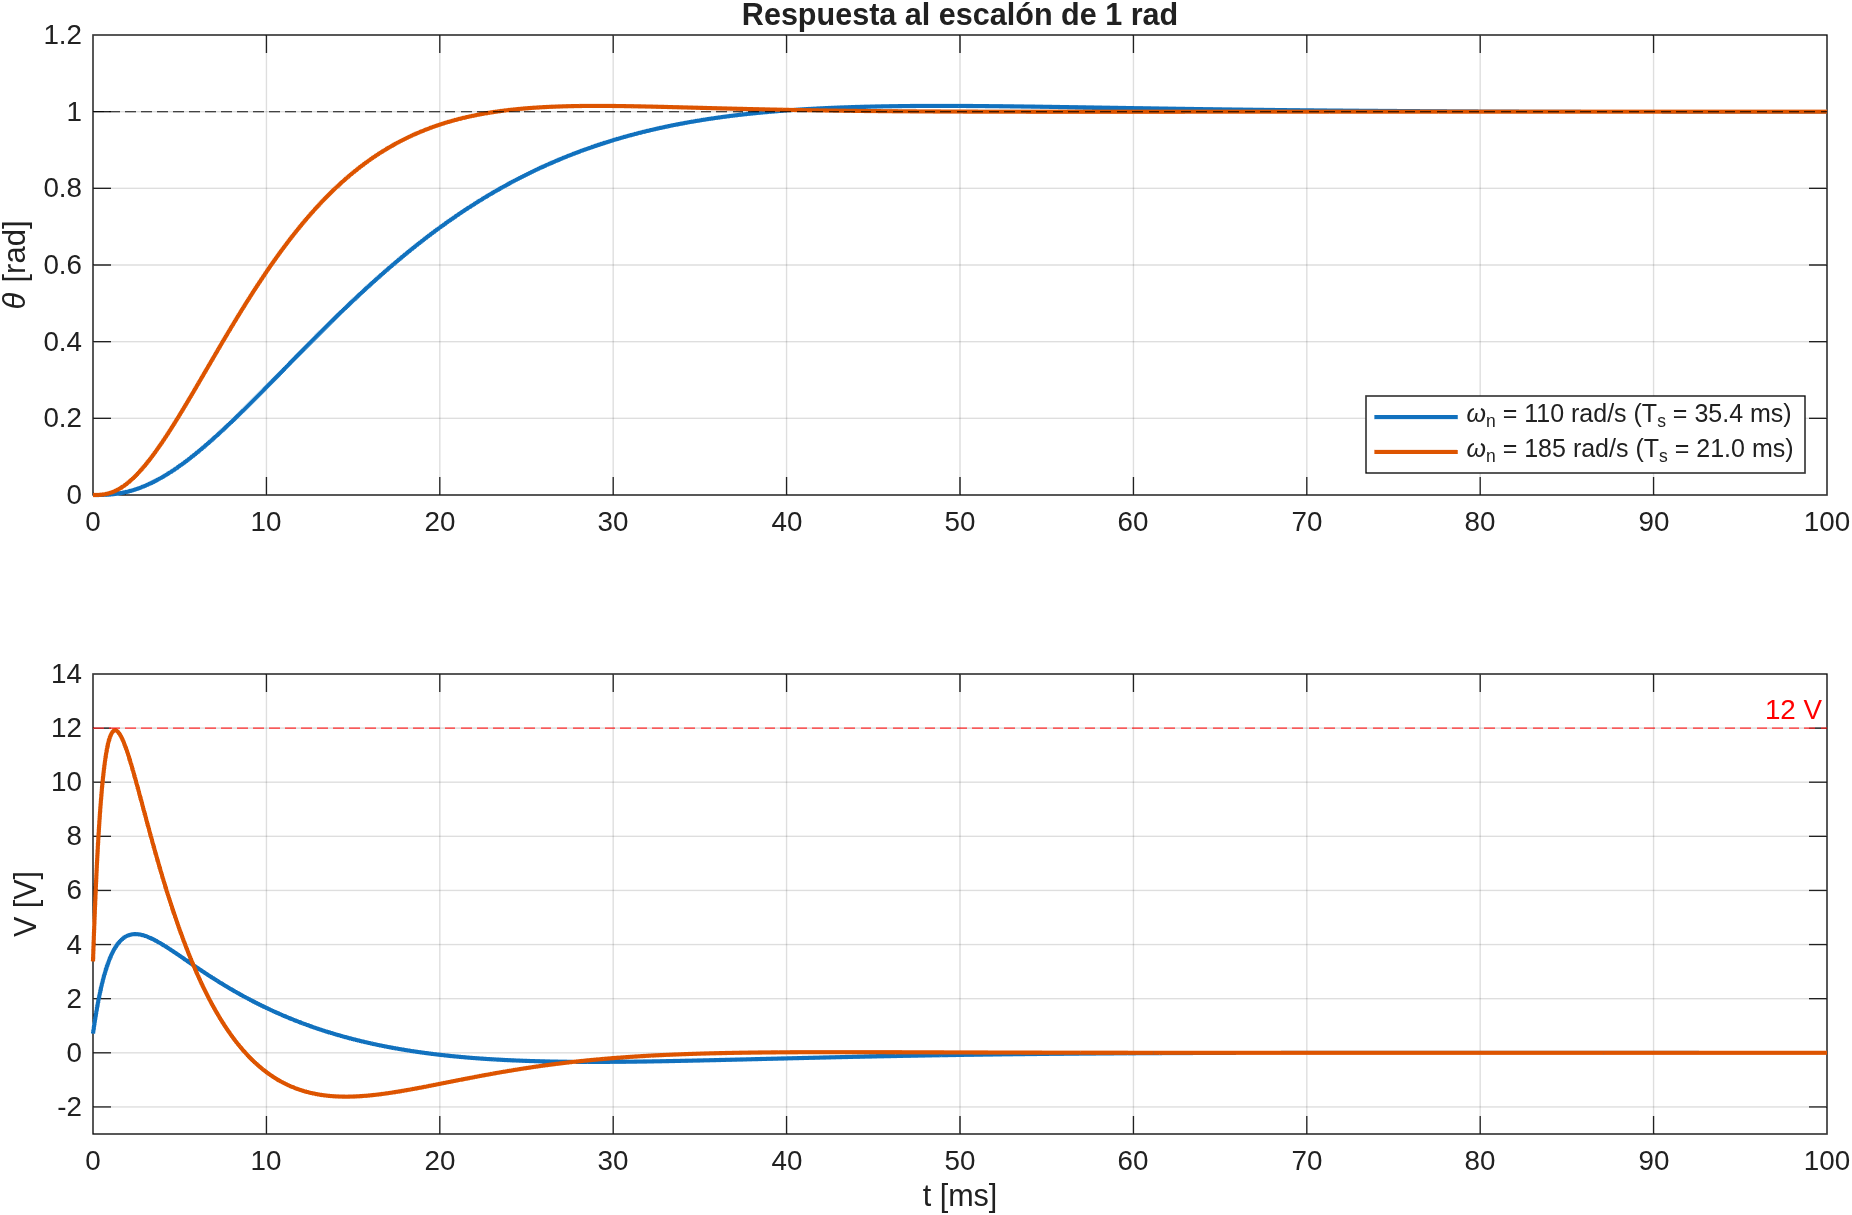
\includegraphics[width=\linewidth]{punto4_theta_V.png}
    \end{column}
    \begin{column}{0.38\textwidth}
      \small
      \textbf{Diseño $\omega_n = 110$} (azul)
      \begin{itemize}
        \item $T_s = 35{,}4$ ms, $PO = 1{,}5$\,\%, $e_{ss}=0$
        \item $|V|_{\text{máx}} = 4{,}39$ V
      \end{itemize}
      Cumple todo con margen.

      \vspace{0.6em}
      \textbf{El pico de $V$ no está en $t=0^+$}
      \begin{itemize}
        \item $V(0^+) = k_1 r = 0{,}71$ V.
        \item Después crece porque $-k_3\,i$ suma tensión mientras sube la corriente:
              el máximo está en $t = 2{,}4$ ms.
        \item Hay que verificar $|V|_{\text{máx}}$ simulando, no alcanza con mirar $k_1$.
      \end{itemize}
    \end{column}
  \end{columns}
\end{frame}

% 9 -----------------------------------------------------------------------
\begin{frame}{Menor $T_s$ sin superar 12 V}
  \begin{columns}[c]
    \begin{column}{0.6\textwidth}
      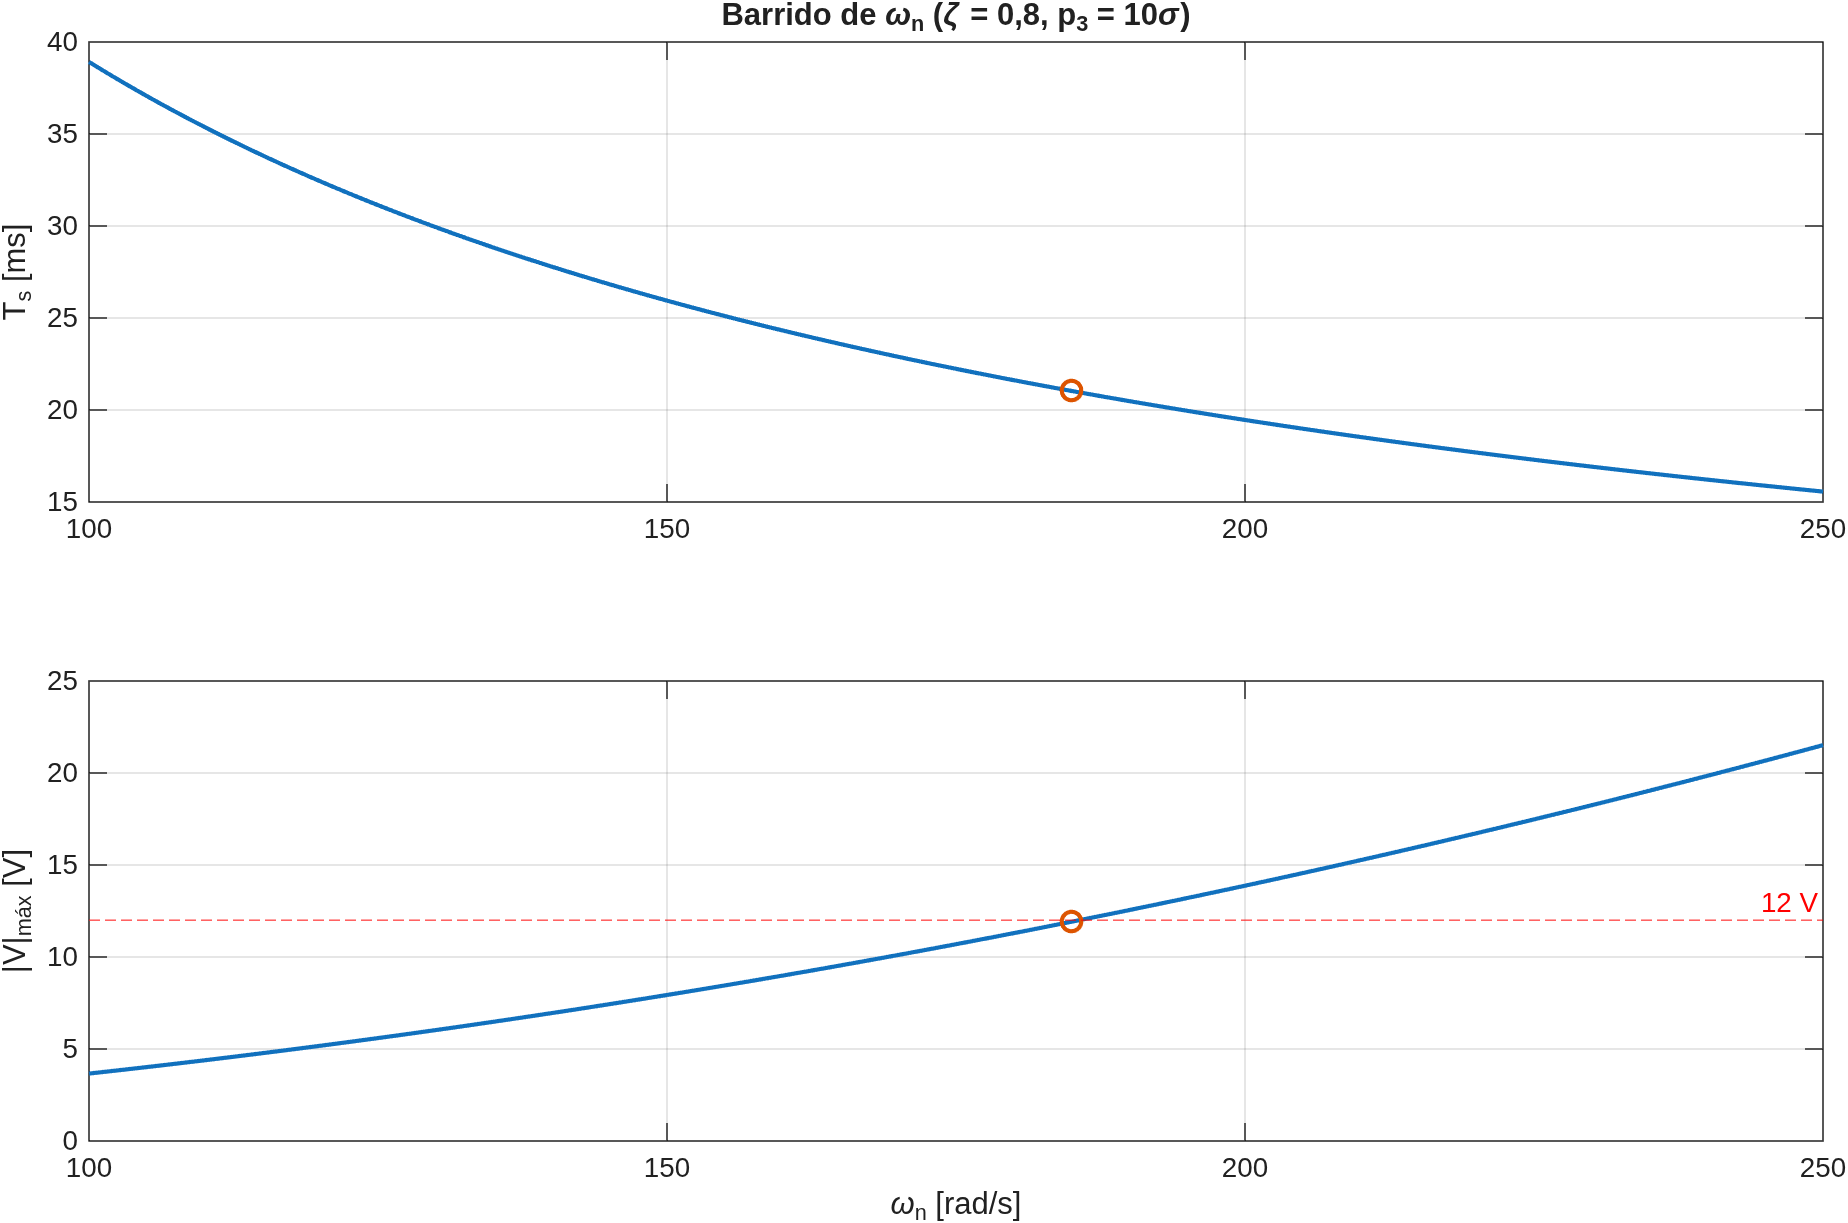
\includegraphics[width=\linewidth]{punto4_barrido_wn.png}
    \end{column}
    \begin{column}{0.38\textwidth}
      \small
      Se mantienen $\zeta = 0{,}8$ y $s_3 = 10\,\sigma$, y se barre $\omega_n$ de 100 a 250 rad/s.
      Para cada $\omega_n$ se recalculan $K$ y $N$, se simula y se mide $T_s$ y $|V|_{\text{máx}}$.

      \vspace{0.6em}
      \textbf{Diseño límite: $\omega_n = 185$ rad/s} (naranja en la diapo anterior)
      \begin{itemize}
        \item $T_s = 21{,}0$ ms, $PO = 1{,}5$\,\%
        \item $|V|_{\text{máx}} = 11{,}92$ V
        \item $K = [3{,}377\ \ 0{,}00139\ \ -2{,}290]$, $N = 3{,}377$
      \end{itemize}
    \end{column}
  \end{columns}
\end{frame}

% 10 ----------------------------------------------------------------------
\begin{frame}{Qué limita el $T_s$}
  \begin{itemize}
    \item Polos más rápidos piden ganancias más grandes, y por lo tanto más tensión:
          \[
            T_s \sim \frac{1}{\omega_n},\qquad |V|_{\text{máx}} \sim \omega_n^2
          \]
          Bajar $T_s$ a la mitad cuesta unas cuatro veces más tensión.
    \item El límite es la \textbf{tensión de la fuente}: por encima de $\omega_n = 185$ rad/s
          el diseño pide más de 12 V.
    \item Si se pidiera más, la fuente saturaría y el lazo dejaría de comportarse como el modelo lineal
          con el que se diseñó: los polos ya no estarían donde se ubicaron.
  \end{itemize}

  \vspace{0.8em}
  \textbf{Resultado}
  \begin{center}
    \begin{tabular}{lcccc}
      \toprule
      Diseño & $T_s$ [ms] & $PO$ [\%] & $e_{ss}$ & $|V|_{\text{máx}}$ [V]\\
      \midrule
      $\omega_n = 110$ & 35,4 & 1,5 & 0 & 4,39\\
      $\omega_n = 185$ (límite) & \textbf{21,0} & 1,5 & 0 & 11,92\\
      \bottomrule
    \end{tabular}
  \end{center}
\end{frame}

\end{document}
